\chapter{Control for \SB{} Locomotion}
\label{controls}

\section{Basic Locomotion Concepts for a Icosahedron Tensegrity Robot}
\label{basic_locomotion}

Locomotion for tensegrity structures like \SB{} is achieved by deforming the structure in a way in which moves the system's center of mass to an unstable configuration, tipping the robot over.
This deformation is usually achieved by either changing the length of the main cable network on the outside of the robot~\cite{sabelhaus2015system,kim2014rapid} or by adding additional cables which run through the structure connecting non-parallel rods~\cite{caluwaerts2014design}.
For the rest of this section, deformation is assumed to be done by actuating the main cable network on the outside of the robot since this is how \SB{} is deformed.

\begin{figure}[thpb]
      \centering
      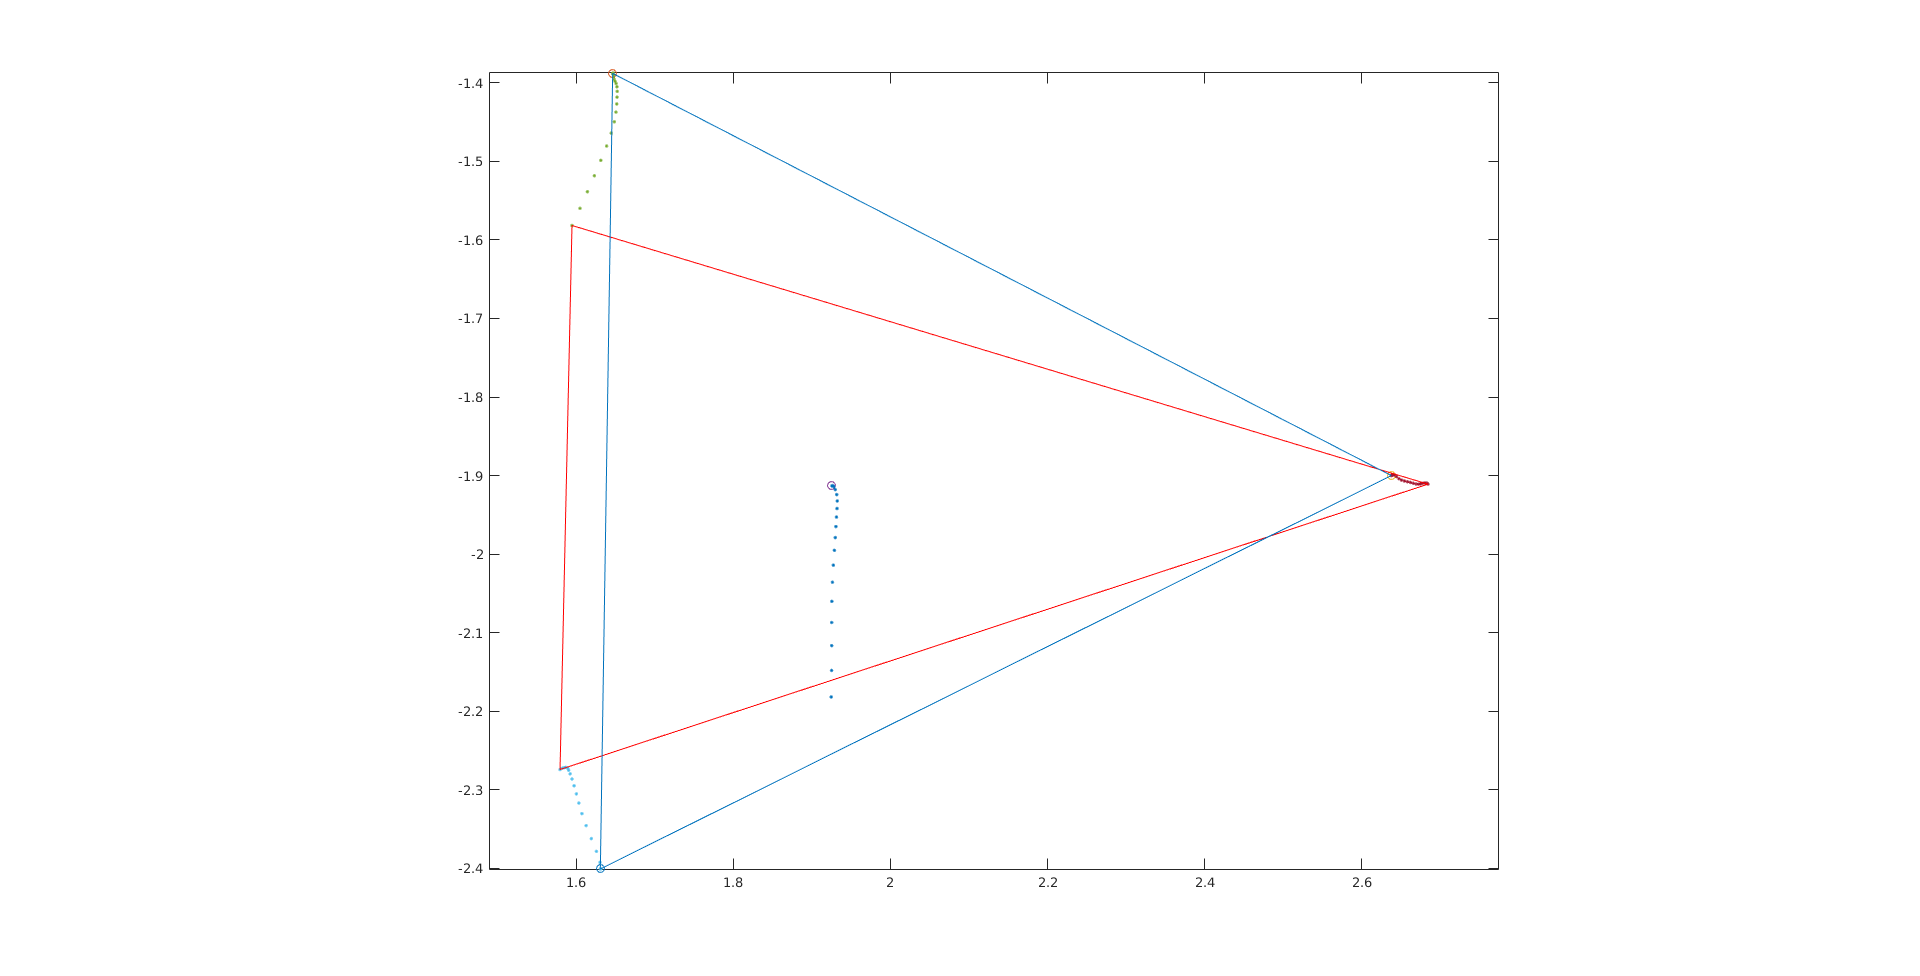
\includegraphics[width=1\columnwidth]{tex/img/Single_flop_bottom_triangle}
      \caption{This is XY data of the bottom triangle of a NTRT simulation of \SB{} performing a single face transition by changing only one side of the bottom triangle.
      No other cable on the system is being actuated during this simulation.
      The red triangle is the bottom triangle at the start of the simulation. 
      The centralized circle represents the center of mass (CoM) of the entire simulated \SB{}. 
      The blue triangle is the configuration where the CoM moves out of the bottom triangle and the robot begins to transition to another face.
      Thus, under ideal conditions and actuation limits, a \SB{} like structure can perform a face transition by the changing of a single cable.}
      \label{fig:single_flop}
\end{figure}

% \SB{} is a tensegrity structure is the shape of an icosahedron.
An regular convex icosahedron is a geometric shape consisting of eight equilateral triangle interlaced with twelve isosceles triangles.
In a passively sable configuration, the bottom of an icosahedron will be resting on either an equilateral or a isosceles triangle.
Utilizing this knowledge, the most simple method for moving the center of mass of an icosahedron can be obtained by changing the length of one side of the bottom triangle to near zero.
This will always move the center of mass to an unstable configuration by effectively reducing the bottom triangle, as seen if figure~\ref{fig:single_flop}, which will cause the robot to transition to another face.
However, this simple control method is not always obtainable on a real robotic system due to limitation on actuation or design methodology.
For \SB{}, this control method is obtainable when the system only has the battery mounted required to actuate the single motor reducing the overall system weight.
Figure~\ref{fig:superball_flop_flat} shows this single motor face transition on a weight reduced \SB{}.

\begin{figure}[thbp]
    \centering
    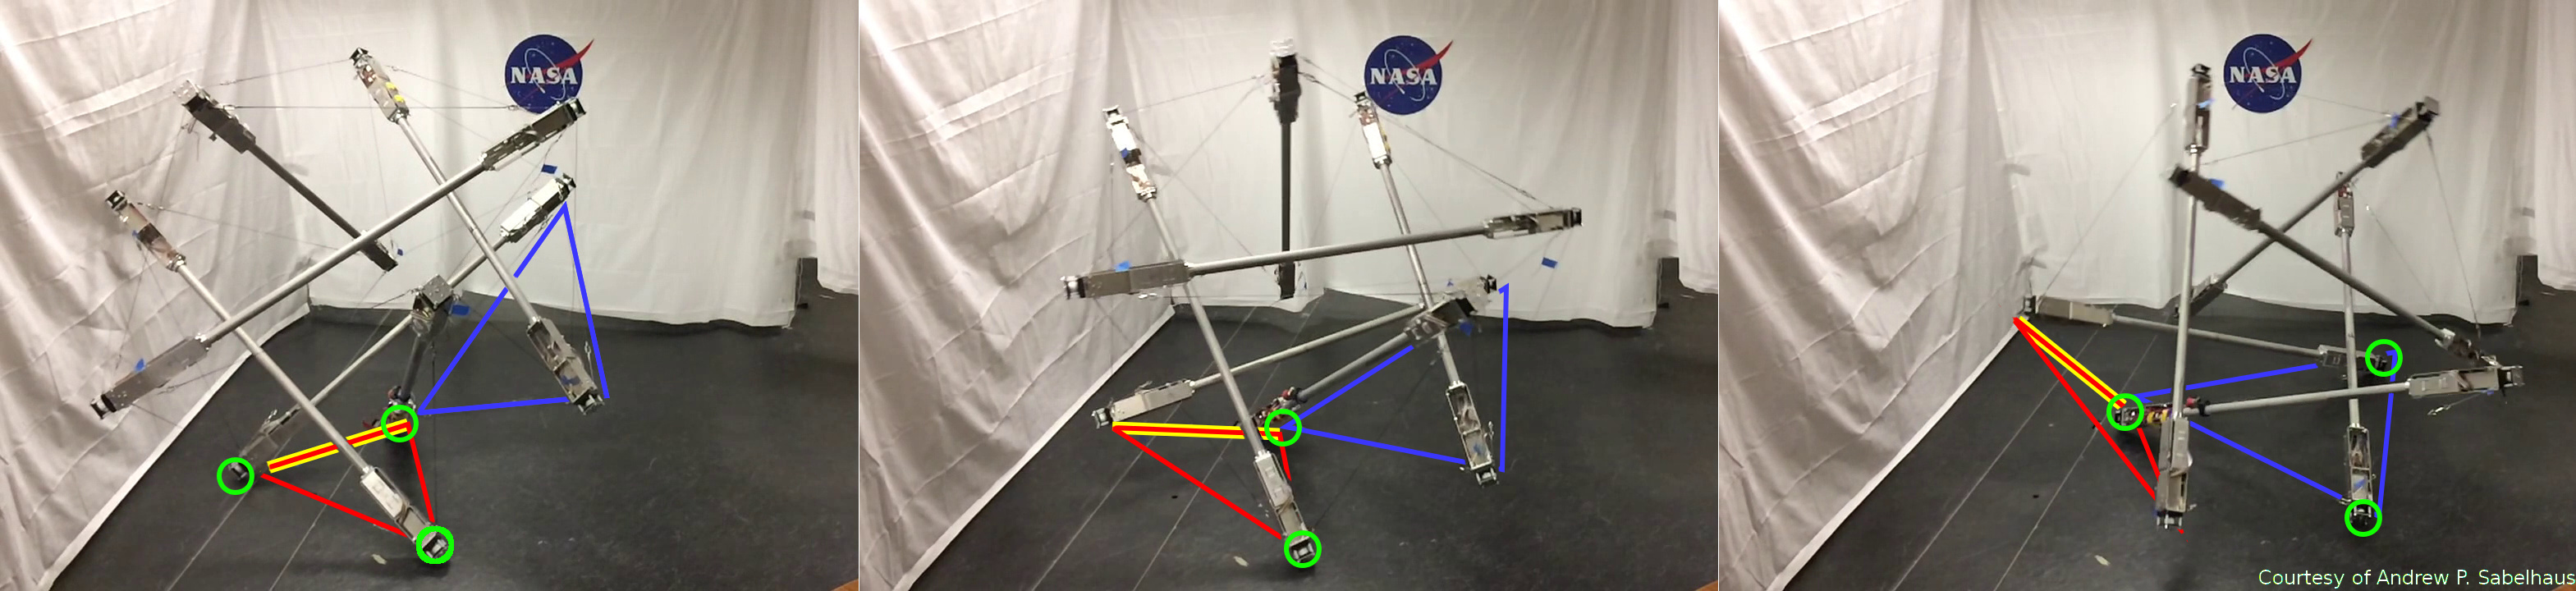
\includegraphics[width=1\linewidth]{tex/img/superball_flop_combined_betterlabels}
    \caption{\SB{} performing a single face-change movement, from one equilateral triangular face to another. The robot begins with all MTRs of the red triangle touching the ground. Then, \SB{} retracts the yellow-highlighted cable on the red triangle, inducing movement. Frame 2 shows \SB{} halfway through the movement with only two points of contact on the ground. Finally, frame 3 shows \SB{} at the end, with all 3 points of the blue triangle in ground contact.}
    \label{fig:superball_flop_flat}
\end{figure}

\SB{} is an underactuated icosahedron tensegrity robot.
Of the 24 connection cables, \SB{} only has 12 cables which are actively actuated and the other cables are passive as discussed in section~\ref{design}.
Since each MTR is manufactured with the same elements, each of the four cables attached to it are one of four types: an actuated cable attached to a motor, an actuated cable from an adjacent MTR terminating at this MTR, a passive cable attached to a spring, or a passive cable from an adjacent MTR terminating at this MTR.
Therefore, there is a unique pattern of cables, and care is needed when choosing this pattern for locomotion. 

For \SB{}, a symmetric pattern is used where each equilateral triangle has at least one actuator associated with one of its sides.
As stated in section~\ref{design}, \SB{} has eight equilateral triangles, so at most three triangles will have more than one actuated side.
These triangles are evenly spaced round the surface of the robot such that there are "rings" of six equilateral triangles with the other two triangles flanking this ring.
Forward locomotion is then achieved by transitioning the structure such that each of the six equilateral triangles on this "ring" come in complete contact with the ground at some instantaneous point in time.
Since a symmetric pattern was desired, it was chosen to placing one actuator per "ring" triangle in such a way where the theoretical full acutation length change of that triangle side would cause the robot to transition towards the next sequential equilateral triangle on that "ring".
The other six motors where then attached as all the side of the remaining two equilateral triangles, those not associated with the "ring".
Figure~\ref{fig:actuator_pattern} (a) shows a graphical overlay of the actuation "ring" and the fully actuated triangles marked in red and blue, respectively.
Figure~\ref{fig:actuator_pattern} (b) is a icosahedron rolled out to show the "walking" gait pattern achieved by rolling about the actuation "ring".

\begin{figure}[thbp]
    \centering
    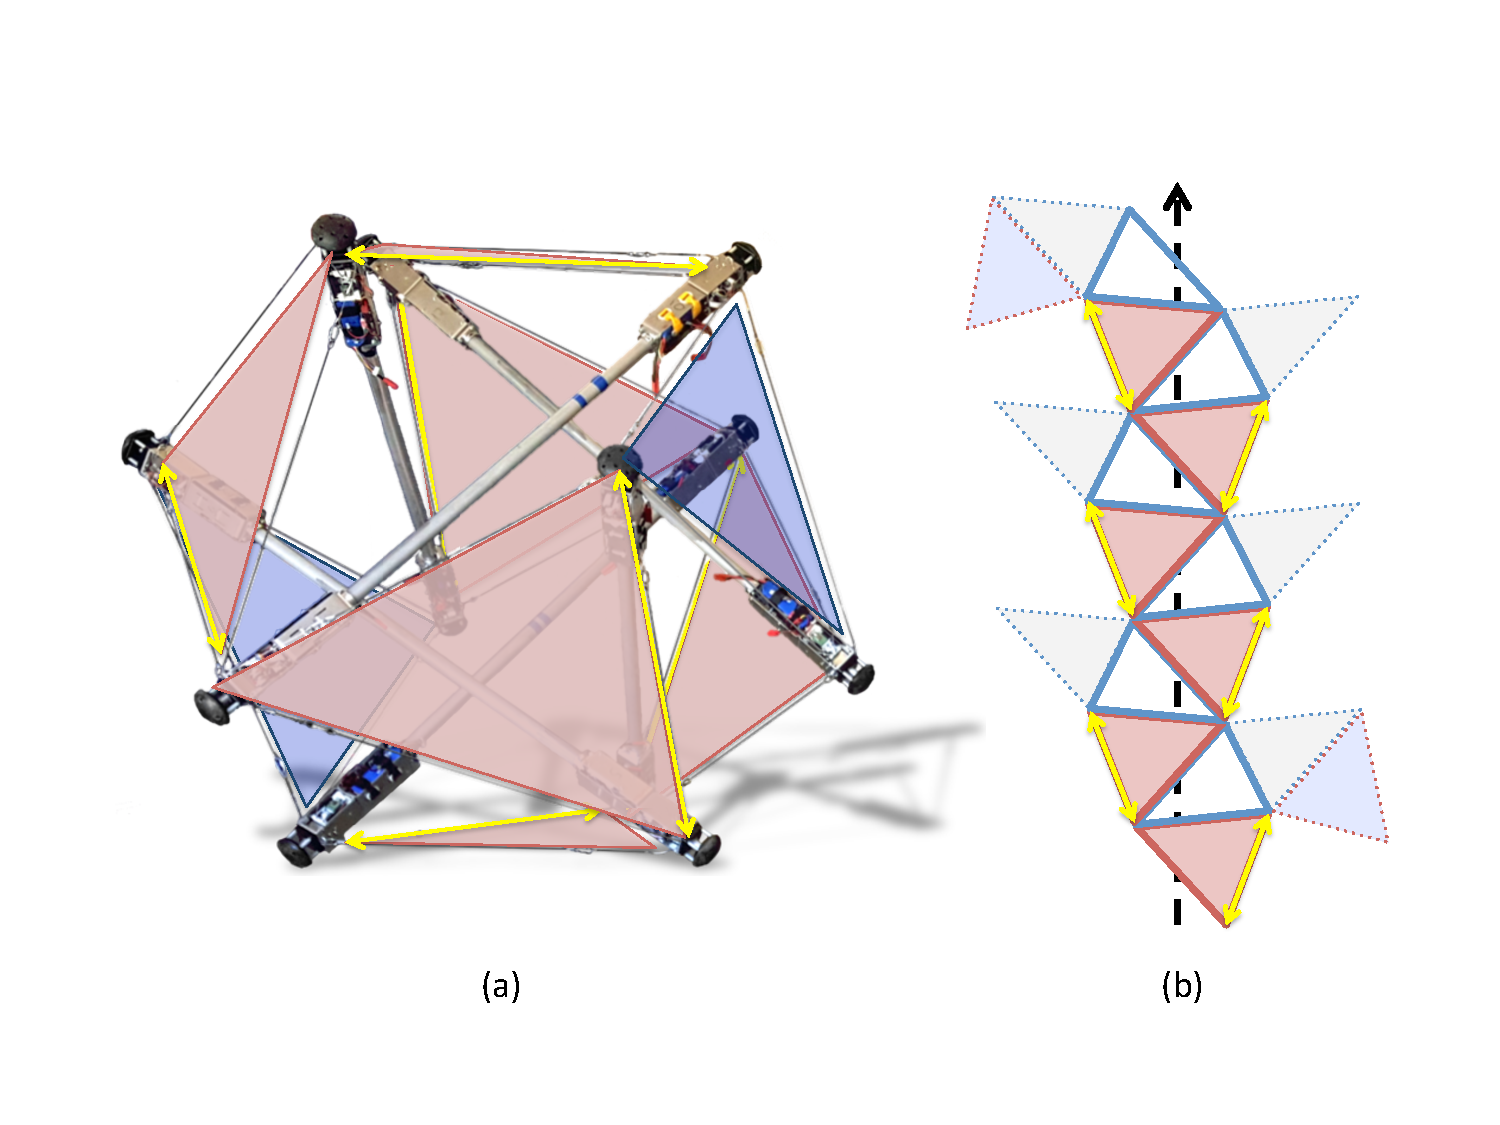
\includegraphics[width=0.8\linewidth]{tex/img/SB_RedvBlue_with_Walk}
    \caption{This image shows the actuation pattern used on \SB{}. There are 8 equilateral triangles, shown in either red or blue. Each red triangle represents a face with only one of the three cable sides actuated. These actuated cables are noted by the yellow double arrows. Each blue triangle, which are not  has actuators on all three cable sides. The basic forward rolling of \SB{} has the robot landing with a red triangle fully on the ground during locomotion. Blue triangles don't touch the ground during this forward rolling pattern. Figure (a) shows each triangle highlighted on \SB{} and figure (b) shows the forward locomotion pattern, or walking pattern, of \SB{}.}
    \label{fig:actuator_pattern}
\end{figure}


% There has been many open loop control techniques that explored this concept through the use of form finding static poses~\cite{}\textcolor{red}{bliss, mirats-tur}.
% Their simulation results show some very promising results for locomotion of variou
% xKim et al~\cite{kim2015robust} developed a method which address some of these issues, but requires .... \textcolor{red}{something non-ideal}.
% However, these techniques do not generalize well to ill-formed robot parameters between simulation and a physical robot, and usually constrain the search space to small manifolds for valid structure configurations.
% When the manifolds are expanded, the search space can become very large resulting in slow results that require a large number of 

% \textcolor{blue}{write about Atil's work and Brian's.}


%Another interesting point could be made about there being two classes of tensegrity robots.  Many of the early approaches stemmed directly out of the modeling and mathematics of static tensegrity structures, which used low-creep cables for stability, and such designs result in very small manifolds of valid structures, with many of the changes in cables lengths resulting in the robot becoming unstable and collapsing as there was no valid equilibrium pose.

\section{Hand-Tuned Stepwise Controller}
\label{hand_stepwise}
The initial controller developed for \SB{} was a basic open loop, hand tuned controller.
Motor position commands where systematically found through experimentation which moved the robot into a kinematically unstable configuration for each of the six faces mentioned in section~\ref{basic_locomotion}.
Under normal conditions on flat ground, when the system starts on an equilateral triangle the forward momentum of the structure after deformation will push it through the isosceles triangle and come to rest on another equilateral triangle.
Using this assumption, only six different kinematic configurations where implemented.
To automate this process, enabling the system to detect which face it resided on was necessary.
A simple K-nearest neighbor algorithm was implemented on recorded IMU data for each equilateral triangle face of \SB{}.
Since the faces are discrete enough, one hundred percent classification was found.
With this information, a basic open loop controller was written that used the detected face as an input and commanded the correct motor commands for the kinematically unstable configuration to transition the robot to the next face.
Once the robot acted the kinematically unstable configuration, all motor commands were set back to their starting configuration.
This ensured correct detection and transition time for the next cycle.
The hand-tuned stepwise controller has two main states, a detect and move state and a relax state as seen in~\ref{fig:stepwise_fsm}.
The transition between each state is time based, where the timing between states was empirically obtained to ensure transition and dynamic settling.

\label{hand_stepwise}
\begin{figure}[thpb]
      \centering
      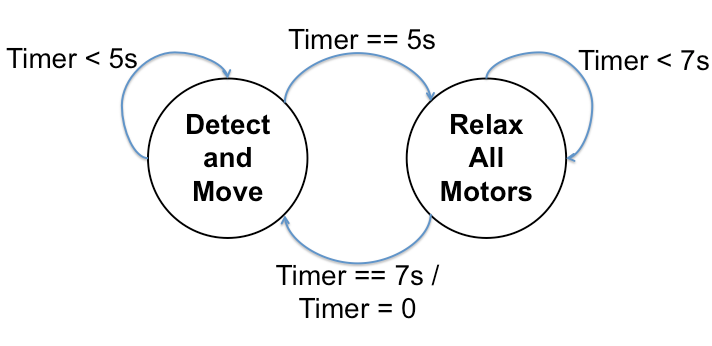
\includegraphics[width=0.7\columnwidth]{tex/img/Stepwise_state_machine/Slide1_fixed}
      \caption{Time based state machine which automates the hand-tuned stepwise controller. Timers are used to allow for dynamic settling before the next action is taken.}
      \label{fig:stepwise_fsm}
\end{figure}

% \section{Learned Neural Net Controller using Guided Policy Search}
% \label{learning_nn_gps}

\todo{incorporate better}
\subsection{Mirror Descent Guided Policy Search}
\label{sec:mdgps}

%Policy search algorithms aim to find a good policy by directly searching through
%the space of policy parameters. 
Guided Policy Search utilizes supervised policy learning to leverage a series of non-generalized optimized local polices to learning a generalizable global policy~\cite{lk-gps-13}.
These non-generalized optimized local policies, $\trajdist_i(\at|\st)$, only successfully work from specific initial states and require full state information.
Guided Policy Search allows for the use of simple and efficient methods for training the local policies,
such as trajectory optimization methods when there is a known model, or
trajectory-centric reinforcement learning methods~\cite{la-lnnpg-14}.

In this work, a modified version of Guided Policy Search is used based on mirror descent~\cite{ml-gpsam-16}, called Mirror Descent Guided Policy Search (MDGPS).
This version optimizes the global policy by sampling the current iteration's local polices and approximates the minimum divergence between the global policy and the local policies.
To optimize the local polices, $\return(\params)$ is minimized such that there is a bound on the Kullback–Leibler divergence (KL-divergence) between the local policy and the linearized global policy $\bar\policy_{\params{i}}$~\cite{bagnell2003covariant,ps-rlmsp-08,pma-reps-10,slmja-trpo-15}.
For clarification, the KL-divergence is a measure of how much information is lost when using a probability distribution to approximate another distribution.
A generic MDGPS algorithm is shown in Algorithm~\ref{alg:mdgps}.

Policy learning machine learning algorithms, commonly called policy search algorithms, are used to directly search the policy parameter space and are alternatives to value function based reinforcement learning algorithms~\cite{bagnell2003policy}. 
%Formally, we wish to find a setting of the
This algorithm tries to find a set of
policy parameters $\params$ which optimizes the policy
$\policy_{\params}(\at|\obs_t)$ with respect to the expected cost. 
%In the finite-horizon episodic setting,
With a finite set of episodes, 
the expected cost under the policy is given by
$\return(\params)=\sum_{t=1}^{T}\mathbb{E}_{\policy_{\params}}[\cost(\st,\at)]$,
where $\cost(\st,\at)$ is the cost function. 
%Here $\st$ denotes the state of our
$\st$ is the state of the
system at time $t$, $\obs_t$ is the observation of the state at time $t$,
and $\at$ is the action at time $t$.

%Guided policy search algorithms use supervised learning to train the policy,
%with supervision coming from several local policies $\trajdist_i(\at|\st)$ that
%are optimized to succeed only from a specific initial state of the task using
%full state information. 
% This is much simpler than the goal of the global
% policy, which is to succeed under partial observability from any initial
% condition sampled from the initial state distribution. These simplifications
% allow the use of simple and efficient methods for training the local policies,
% such as trajectory optimization methods when there is a known model, or
% trajectory-centric reinforcement learning methods~\cite{la-lnnpg-14}. 

% In this work, the 
% The specific algorithm used in this work is MDGPS, which interprets GPS as
% approximate mirror descent on $\return(\params)$~\cite{ml-gpsam-16}. The local
% policies are optimized to minimize $\return(\params)$ subject to a bound on the
% KL-divergence between the local policy $\trajdist_i$ and the linearization of
% the global policy $\bar\policy_{\params{i}}$, following previous
% work~\cite{bagnell2003covariant,ps-rlmsp-08,pma-reps-10,slmja-trpo-15}.
% Optimizing the global policy is done using the samples collected in the current
% iteration, which are used in a supervised fashion to approximately minimize the
% divergence between the global policy and the local policies.

\setlength{\textfloatsep}{12pt}
\begin{algorithm}[tb]
    \caption{Mirror descent guided policy search (MDGPS)}
    \label{alg:mdgps}
    \begin{algorithmic}[1]
        \FOR{iteration $k = 1$ to $K$}
            \STATE Run either each $\trajdist_i$ or $\policy_{\params}$ to
            generate samples $\{\traj\}$
            \STATE Set
            $\trajdist_i\leftarrow\argmin_{\hat\trajdist_i}\mathbb{E}_{\hat\trajdist_i}[\cost(\traj)]~s.t.~D_{KL}(\hat\trajdist_i\|\bar\policy_{\params{i}})\leq\epsilon$
            \STATE Train $\policy_{\params}$ using supervised learning on
            $\{\traj\}$
        \ENDFOR
    \end{algorithmic}
\end{algorithm}

% The generic MDGPS algorithm is summarized in Algorithm~\ref{alg:mdgps}. On line
% 2, samples are collected by running either the global policy or the local
% policies. This choice between ``on-policy'' and ``off-policy'' sampling is
% detailed in previous work~\cite{ml-gpsam-16}. On line 3, the algorithm improves
% the local policies using an LQR-based update using fitted local linear models:
% the samples are first used to fit time-varying linear dynamics for each local
% policy, and these fitted dynamics are then used with a KL-constrained LQR
% optimization to update the linear-Gaussian local policies. This corresponds to a
% simple model-based trajectory-centric reinforcement learning method, and further
% details can be found in prior work~\cite{la-lnnpg-14}. On line 4, the global
% policy $\policy_\params(\at|\st)$ is updated using supervised learning, with the
% training data corresponding to the states along the samples, with actions given
% by the new updated local policies. This causes the global policy to ``catch up''
% to the newly improved local policies, improving its behavior for the next
% iteration.


\section{Optimizing Periodic Gaits with MDGPS}
\label{sec:chains}

Using the MDGPS method stated in section~\ref{sec:mdgps}, a periodic rolling gait for \SB{} was learned using single transitions between faces mentioned in section~\ref{basic_locomotion} as the local policies and how to transition between them using limited sensor data as the global policy. 
In order to obtain this stable periodic rolling gait, the task is split across several policies, each optimized over a small time segment.
After establishing a desired behavior across the states seen by the policies, a global policy is learned that can generalized the behavior of the local polices based on the Guided Policy Search framework.

% The efficiency and speed of model-based policy optimization methods, such as the
% LQR-based method used to optimize the local policies in MDGPS, is due in large
% part to the fact that dynamic programming can allow for large changes to a
% policy that would be impractical with purely sample-based model-free
% methods~\cite{la-lnnpg-14}. However, in complex stochastic domains, such as the
% contact-rich dynamical system of a rolling tensegrity robot, the accumulation of
% uncertainty and variability under an unstable policy can make it difficult to
% apply dynamic programming over the long horizons needed to establish a periodic
% gait. We demonstrate this effect through our experimental results in
% Section~\ref{sec:simresults}. 
% In this section, we describe how we can obtain a
% policy with stable periodic behavior by first splitting the task across multiple
% policies, each optimized over a smaller time segment where it is easier to apply
% dynamic programming, and establishing good behavior across the range of states
% visited by these policies. Following the framework of GPS algorithms, we
% subsequently learn a global policy that can generalize the behavior of the local
% policies and encapsulate a successful periodic gait into a single policy.

GPS algorithms such as MDGPS use supervised learning to learn a global policy,
where the supervision comes from several local policies $\trajdist_i(\at|\st)$,
$i\in\{1,\ldots,C\}$. Each local policy is trained from a different initial
state, where $C$ is the chosen number of initial states. Each local policy is
optimized over $T^{\trajdist}$ time steps, and we wish to learn a global policy
$\policy_{\params}(\at|\obs_t)$ that can succeed by generalizing the behavior of
these local policies over an episode of length $T^{\policy}$.

In locomotion
tasks, we ideally want the global policy to exhibit continuous successful
behavior, i.e., $T^{\policy}=\infty$, and we can empirically determine
$T^{\trajdist}$ based on the amount of supervision the global policy needs to
learn a continuous periodic gait.
For \SB{}, $T^{\trajdist}$ is initialized to a short horizon, and continually increased 
until the global policy learns a successful locomotion gait.

If the required $T^{\trajdist}$ is long, as is the case for the \SB{} locomotion
task, it is difficult to optimize a local policy over this time horizon due to
the accumulation of uncertainty and errors. 
However, $L$ local policies $\trajdist_i^1,\ldots,\trajdist_i^L$ can be learned for each
initial state $i$, each optimized for $T^{\trajdist}/L$ time steps. For the
local policies $\trajdist_i^j$, $j\in\{2,\ldots,L\}$, we set the initial state
$\state_0^j$ to be the final state of the preceding local policy, i.e.,
$\state_{T^{\trajdist}/L}^{j-1}$. This amounts to training local policies in a
sequential fashion, where the $L$ local policies together are optimized over
$T^{\trajdist}$ time steps.
The algorithmic details using in learning a periodic stable gait for \SB{} can be seen in Algorithm~\ref{alg:mdgpsseq}.
Note that on line 7, samples can be collected from either the local polices or the global policy.
Initially, these samples are taken from the local polices, but are switched to the global policy based on a user's expert knowledge for how the local polices are performing.

% In previous work, the motivation behind choosing multiple initial states was so
% that the global policy could succeed from all of these initial states, and
% ideally generalize to other initial states as well~\cite{lfda-eetdv-16}. 
% In our
% work, we found that choosing multiple initial states is also beneficial in
% learning a stable periodic gait compared to having just one initial state, and
% Section~\ref{sec:simresults} demonstrates this difference. The reason for this
% is that, to achieve the same amount of supervision using only one initial state,
% the sequence of local policies $\trajdist_1^1,\ldots,\trajdist_1^L$ must be much
% longer, and training a longer sequence increases the chances of divergence and
% instability in the behavior of the local policies compared to training shorter
% sequences from several stable initial states.

\setlength{\textfloatsep}{12pt}
\begin{algorithm}[tb]
    \caption{MDGPS with sequential local policies}
    \label{alg:mdgpsseq}
    \begin{algorithmic}[1]
        \FOR{iteration $k = 1$ to $K$}
            \FOR{$i = 1$ to $C$}
                \STATE $S_i\leftarrow\{\}$
                \FOR{the desired number of samples}
                    \STATE $x_0\leftarrow$ initial state $i$
                    \FOR{$l = 1$ to $L$}
                        \STATE Run either $\trajdist_i^l$ or $\policy_{\params}$ to
                        generate sample $\traj$
                        \STATE $S_i$, $x_0\leftarrow{S_i}\cup\{\traj\}$, end state of $\traj$
                    \ENDFOR
                \ENDFOR
                \FOR{$l = 1$ to $L$}
                    \STATE $\trajdist_i^l\leftarrow\argmin_{\hat\trajdist_i^l}\mathbb{E}_{\hat\trajdist_i^l}[\cost(\traj)]~s.t.~D_{KL}(\hat\trajdist_i^l\|\bar\policy_{\params{i}})\leq\epsilon$
                \ENDFOR
            \ENDFOR
            \STATE Train $\policy_{\params}$ using supervised learning on
            $\bigcup_iS_i$
        \ENDFOR
    \end{algorithmic}
\end{algorithm}

% Our method is detailed in Algorithm~\ref{alg:mdgpsseq}. On line 7, we collect
% samples from either the local policies or global policy. In our work, we start
% by sampling from the local policies, and we switch to sampling from the global
% policy after a fixed number of iterations, which we set empirically based on the
% performance and stability of the local policies. On line 8, we store the
% collected sample, and in order to run the policies sequentially, we set the
% starting state of the next policy to be the end state of the sample $\traj$
% collected from the current policy. Aside from this difference in sampling, the
% rest of the algorithm is identical to MDGPS.


% \section{Learning Locomotion for \SB{}}
% \label{sec:superball}

% For \SB{} locomotion, we chose six initial states that correspond to the stable 
% ground faces that the robot traverses when rolling forward. These faces are natural 
% and stable initial states that the robot may start from. We set $T^{\trajdist}=100$ and
% $L=2$, so from each initial state $i$, two local policies $\trajdist_i^1$ and
% $\trajdist_i^2$ are optimized over 50 time steps each, where each time step is
% \SI{0.1}{\second}. We found that a fully optimized local policy can perform
% about two transitions from one ground face to the next face over 5 seconds. We
% also found it helpful in our work to not begin training $\trajdist_i^2$ until
% $\trajdist_i^1$ trains for several iterations, so that $\state_{50}^1$, which is
% $\state_0^2$, is more stable and has lower variance.  We show in
% Section~\ref{sec:simresults} that training two local policies in this fashion is
% much more sample efficient than training one local policy for 10 seconds, and
% produces smoother and faster rolling behavior. In total, in our work, 12 local
% policies are trained in sequences of two, and this provided the global policy
% the supervision required to learn to roll continuously.

\subsection{Kinematic Constraints for Safe Actions}

A challenge for machine learning techniques is that policy requirements are usually encoded into the techniques unique cost function.
This function not only needs to guide task level objectives, such as movement, but without any other external limits the cost function must also guide hard constraints like safety.
Due to the fact that \SB{} only has position control, as outlined in section~\ref{sec:cable_tension}, a random sampling of motor position might cause the system to tension a cable beyond it's mechanical limit breaking the cable, the motor, or both.
These configurations of tension limits are difficult to to embed analytically into the cost function and even harder to optimally balance with task level objectives.
Thus, a simple global motor position safety constraint method was implemented that interfaces outside of the machine learning framework.

% One of the challenges with automated policy learning is that all requirements
% for the policy are generally encoded in the cost function, including task-level
% objectives such as desired rolling direction and hard constraints such as
% safety. Due to the structure of tensegrity systems, unsafe actuation of the
% motors can place the robot into configurations with unacceptable risk of cable
% or motor failure. The configurations associated with such high-tension
% conditions are difficult to encode analytically and even more difficult to
% balance against primary task objectives in the cost function. We therefore adopt
% a simple safety constraint approach to enable safe learning and policy execution
% on the \SB{} hardware. This approach is challenging to use with hand-engineered
% policies, which often exploit unsafe but effective actions to quickly yield a
% locomotion gait. However, the approach is much easier to adopt with learned
% policies, as it naturally embeds itself into the training procedure.

Specifically, the cable tensions are estimated for a particular set of actuator positions using a simple forward kinematic model of \SB{}.
This model is based the model outlined in section~\ref{sec:dynamic_modeling_sb} with the simplification of no gravity or ground contact.
The limits are preset as a maximum tension value exerted on any cable based on a user defined maximum value.
For \SB{}, this maximum value was experimentally found to be \SI{250}{\newton}.
Computing the cable tensions for a given set of motor positions takes a few milliseconds using forward
kinematics. As this is easily parallelized, a database was constructed containing
about 100 million motor positions deemed safe in a few hours.
Then, when the policy outputs an action, an efficient look up method called Fast
Library for Approximate Nearest Neighbors (FLANN)~\cite{flannsoftware} is used to compute
and command the nearest ($\cost_1$ norm) safe action.
This ensures that even if the exact action isn't located in the table, an approximate action set is chosen.
At runtime, finding the nearest neighbor action takes roughly \SI{200}{\micro\second} and is
easily embedded into both training and testing without disrupting the command
frequency of \SI{10}{\hertz}.

% Specifically, we estimate the cable tensions for a particular set of actuator
% positions using a simple forward kinematics model of \SB{}.  We repeat this
% process for many different randomly generated motor settings and store all sets
% of motor positions for which all cable tensions of the robot are below the
% acceptable threshold. Then, when the policy outputs an action, we use the Fast
% Library for Approximate Nearest Neighbors (FLANN)~\cite{flannsoftware} to compute
% and command the nearest ($\cost_1$ norm) safe action. Computing the cable tensions
% for a given set of motor positions takes a few milliseconds using forward
% kinematics. As this is easily parallelized, we constructed a database containing
% about 100 million motor positions deemed safe in a few hours. At runtime,
% finding the nearest neighbor action takes roughly \SI{200}{\micro\second} and is
% easily embedded into both training and testing without disrupting the command
% frequency of \SI{10}{\hertz}.

% By separating this safety constraint from the cost function, we avoid the need
% to tune the parameters of the cost function to weigh the opposing objectives of
% speed and hardware safety. Furthermore, we encode safety as a hard constraint
% using this method, and we directly prevent unsafe actions rather than just
% penalizing them. Utilizing these kinematic constraints is extremely helpful in
% transferring policies learned in simulation directly onto the real robot. In
% simulation, the physical limits are less restrictive, and going beyond the safe
% limits does not have any adverse effects, so it is possible to train a policy
% that exploits these inaccuracies in order to succeed. We can make sure this does
% not happen by enforcing stronger constraints of what actions the policy can
% output, and it is more likely that the policy trained with these constraints in
% simulation will not fail on the real robot, or even worse, cause damage and
% hardware problems.

\subsection{Generalization Across Domains}

Because we train local policies with full state information $\st$ but learn a
global policy that only receives an observation of the state $\obs_t$ as input,
we are able to train a global policy that operates under partial observability
at test time while maintaining the simplicity of training the local policies on
the full state. This separation between the local policies and global policy
reflects prior work on tasks involving partial observability, where the
intuition is that the local policies are trained in a controlled environment but
the global policy must be able to adapt to a more general
setting~\cite{lfda-eetdv-16}.

In our case, the full state $\st$ can only be obtained through either simulation
or the use of an external state estimator system on the physical \SB{}
robot~\cite{caluwaerts2016esitmation}. In contrast, we choose an observation
$\obs_t$ that can be calculated directly from the sensors on the robot itself.
This greatly simplifies the transfer from simulation to the real robot, as the
learned policy is less prone to overfit to the simulation and takes actions
directly based on the sensor measurements from the physical robot. Furthermore,
because the goal of \SB{} and many other robots is deployment to
unfamiliar, remote environments, the choice of an observation that relies only
on the robot's onboard sensors is very important, as it is unrealistic to expect
the level of information and reliability that an external state estimator can
provide. For a description of the state and observation, as well as the details
and dimensionalities of the sensors, see Section~\ref{sec:setup}.

Because the real-world sensors and actuators are noisy and imperfect, we attempt
to model this in simulation by introducing noise on the input to the policy
during training. We model measurement errors and sensor inaccuracies by adding
Gaussian noise with mean 0 and variance equal to 10\% of the range of the
observation. To model sensor failure, latency, and network issues such as
connection errors, we randomly drop observations 10\% of the time. When the
current observation is dropped, the previous observation is used as the input to
the policy. We found that adding noise improves the generalization capabilities
of the learned policy across conditions such as terrain, gravity, and motor
failure, and we test against these conditions in Section~\ref{sec:simresults}.

\section{Experimental Results}
\label{sec:results}

In our experiments, we aim to answer several questions. First, can we learn
policies in simulation that allow the simulated \SB{} to roll efficiently
under
various settings of terrain, gravity, sensor noise, and robot parameters?
Second, do our learned feedback policies generalize better to changes in
environmental and robot parameters compared to open-loop learned policies? 
Finally, can we transfer the learned policy from
simulation to the real robot, and have the real robot roll?

In Section~\ref{sec:simresults}, we establish the benefits of our method for
training sequential local policies, as well as initializing from multiple
initial states. We then test in simulation the efficiency of the learned
policies and make comparisons to establish the importance of learning and
feedback. In Section~\ref{sec:realresults}, we evaluate a learned policy on the
real robot.

\subsection{Experimental Setup}
\label{sec:setup}

We encode the state of the system $\st$ as the position and velocity of each of
the 12 bar endpoints of \SB{}, and the position and velocity of each of the 12
motors, measured in radians, for a total dimensionality of 96. We experimented
with two different representations for the observation $\obs_t$. The ``full''
36-dimensional observation includes motor positions, and also uses elevation and
rotation angles calculated from the accelerometer and magnetometer sensors on
the robot. The ``limited'' observation is 12-dimensional and only uses the
acceleration measurement along the bar axis from each of the accelerometers. We
found that interfering magnetic fields near the testing grounds at NASA
Ames cause the magnetometers to be unreliable and difficult to calibrate, and
because of this, the policy using the limited observation is much easier to
transfer on to the real robot. The action $\at$ is the instantaneous desired position 
of each motor. 

For our task, each local policy requires about 200 samples before they are
reliably successful. Simultaneously during training of the local policies, we
learn a global policy, which in our work is a deep neural network with three
hidden layers of 64 rectified linear units (ReLU) each, using the same samples.
Our cost function $l(\st,\at)$ is simply the negative average velocity
of the bar endpoints of the robot, so that the local policies are trained to
roll as quickly as possible.

\subsection{Results in Simulation}
\label{sec:simresults}

\begin{table*}[t]
    \centering
    \resizebox{\textwidth}{!}{%
        \begin{tabular}{|llrrrrr|}
            \hline
            \multicolumn{5}{|c|}{}                                                                                                                                                                                                                                                                                  & \multicolumn{2}{c|}{} \\
            \multicolumn{2}{|c}{}                                                        & \multicolumn{3}{c|}{\multirow{-2}{*}{\textbf{Our Method}}}                                                                                                                                                               & \multicolumn{2}{c|}{\multirow{-2}{*}{\textbf{Open-Loop}}} \\
            \multicolumn{2}{|c}{}                                                        & \multicolumn{1}{r|}{Full Observation,}                                 & \multicolumn{1}{r|}{Limited Observation,}                              & \multicolumn{1}{r|}{Limited Observation,}                              & \multicolumn{1}{r|}{Mean Actions from}                           & Hand-Engineered \\
            \multicolumn{2}{|c}{}                                                        & \multicolumn{1}{r|}{Six Initial States}                                & \multicolumn{1}{r|}{Six Initial States}                                & \multicolumn{1}{r|}{One Initial State}                                 & \multicolumn{1}{r|}{Best Learned Policy}                         & Punctuated Rolling \\
            \cline{3-7}
            \multicolumn{2}{|l}{}                                                        & \multicolumn{1}{r|}{}                                                  & \multicolumn{1}{r|}{}                                                  & \multicolumn{1}{r|}{}                                                  & \multicolumn{1}{r|}{}                                            & \\
            \multicolumn{2}{|l}{\multirow{-2}{*}{\textbf{Normal Conditions}}}            & \multicolumn{1}{r|}{\multirow{-2}{*}{$\mathbf{25.307\pm0.309}$}}       & \multicolumn{1}{r|}{\multirow{-2}{*}{$24.141\pm0.352$}}                & \multicolumn{1}{r|}{\multirow{-2}{*}{$20.008\pm0.871$}}                & \multicolumn{1}{r|}{\multirow{-2}{*}{$\mathit{25.076\pm0.078}$}} & \multirow{-2}{*}{$10.266\pm0.071$} \\
            \rowcolor[HTML]{D3D3D3}
            \cellcolor[HTML]{D3D3D3}                                   & Rocky           & \multicolumn{1}{r|}{\cellcolor[HTML]{D3D3D3}$\mathit{6.025\pm2.835}$}  & \multicolumn{1}{r|}{\cellcolor[HTML]{D3D3D3}$\mathbf{9.568\pm5.197}$}  & \multicolumn{1}{r|}{\cellcolor[HTML]{D3D3D3}$3.124\pm1.083$}           & \multicolumn{1}{r|}{\cellcolor[HTML]{D3D3D3}$3.069\pm2.201$}     & $1.734\pm0.411$ \\
            \rowcolor[HTML]{D3D3D3}
            \cellcolor[HTML]{D3D3D3}                                   & Uphill          & \multicolumn{1}{r|}{\cellcolor[HTML]{D3D3D3}$\mathbf{18.547\pm0.231}$} & \multicolumn{1}{r|}{\cellcolor[HTML]{D3D3D3}$\mathit{16.107\pm0.809}$} & \multicolumn{1}{r|}{\cellcolor[HTML]{D3D3D3}$13.573\pm0.174$}          & \multicolumn{1}{r|}{\cellcolor[HTML]{D3D3D3}$7.721\pm0.236$}     & $8.136\pm0.026$ \\
            \rowcolor[HTML]{D3D3D3}
            \multirow{-3}{*}{\cellcolor[HTML]{D3D3D3}\textbf{Terrain}} & Downhill        & \multicolumn{1}{r|}{\cellcolor[HTML]{D3D3D3}$\mathbf{32.896\pm0.275}$} & \multicolumn{1}{r|}{\cellcolor[HTML]{D3D3D3}$\mathit{29.970\pm0.858}$} & \multicolumn{1}{r|}{\cellcolor[HTML]{D3D3D3}$21.963\pm2.403$}          & \multicolumn{1}{r|}{\cellcolor[HTML]{D3D3D3}$27.661\pm0.136$}    & $11.264\pm0.091$ \\
                                                                       & 10\%            & \multicolumn{1}{r|}{$\mathbf{19.505\pm0.746}$}                         & \multicolumn{1}{r|}{$16.966\pm0.362$}                                  & \multicolumn{1}{r|}{$13.927\pm0.516$}                                  & \multicolumn{1}{r|}{$\mathit{18.024\pm2.356}$}                   & $11.044\pm0.054$ \\
                                                                       & 50\%            & \multicolumn{1}{r|}{$\mathbf{23.331\pm0.871}$}                         & \multicolumn{1}{r|}{$\mathit{21.220\pm0.202}$}                         & \multicolumn{1}{r|}{$17.766\pm0.490$}                                  & \multicolumn{1}{r|}{$19.673\pm3.244$}                            & $10.310\pm0.010$ \\
            \multirow{-3}{*}{\textbf{Gravity}}                         & 200\%           & \multicolumn{1}{r|}{$\mathbf{27.600\pm2.307}$}                         & \multicolumn{1}{r|}{$\mathit{26.715\pm0.566}$}                         & \multicolumn{1}{r|}{$21.680\pm1.330$}                                  & \multicolumn{1}{r|}{$24.865\pm0.190$}                            & $9.845\pm0.009$ \\
            \rowcolor[HTML]{D3D3D3}
            \cellcolor[HTML]{D3D3D3}                                   & Heavy           & \multicolumn{1}{r|}{\cellcolor[HTML]{D3D3D3}$12.521\pm1.710$}          & \multicolumn{1}{r|}{\cellcolor[HTML]{D3D3D3}$\mathbf{14.561\pm0.079}$} & \multicolumn{1}{r|}{\cellcolor[HTML]{D3D3D3}$\mathit{12.972\pm0.110}$} & \multicolumn{1}{r|}{\cellcolor[HTML]{D3D3D3}$1.081\pm0.019$}     & $10.550\pm0.003$ \\
            \rowcolor[HTML]{D3D3D3}
            \multirow{-2}{*}{\cellcolor[HTML]{D3D3D3}\textbf{Robot}}   & End Cap Failure & \multicolumn{1}{r|}{\cellcolor[HTML]{D3D3D3}$\mathit{21.890}$}         & \multicolumn{1}{r|}{\cellcolor[HTML]{D3D3D3}$\mathbf{22.100}$}         & \multicolumn{1}{r|}{\cellcolor[HTML]{D3D3D3}$ $}                       & \multicolumn{1}{r|}{\cellcolor[HTML]{D3D3D3}$10.291$}            & $10.247$ \\
                                                                       & 0\%             & \multicolumn{1}{r|}{$\mathbf{26.494}$}                                 & \multicolumn{1}{r|}{$\mathit{25.828}$}                                 & \multicolumn{1}{r|}{$ $}                                               & \multicolumn{1}{r|}{}                                            & \\
            \multirow{-2}{*}{\textbf{Added Noise}}                     & 20\%            & \multicolumn{1}{r|}{$\mathit{7.725}$}                                  & \multicolumn{1}{r|}{$\mathbf{19.212}$}                                 & \multicolumn{1}{r|}{$ $}                                               & \multicolumn{1}{r|}{\multirow{-2}{*}{N/A}}                       & \multirow{-2}{*}{N/A} \\
            \hline
        \end{tabular}%
    }
    \caption{
        \label{table:distance}
        Average distances in meters traveled using the policies learned through
        our method with varying observation representations and local policy
        training schemes, the open-loop mean actions from the learned policy
        that performs best under training conditions, and the hand-engineered
        open-loop policy. Results are averaged across five trials of one minute
        each for a variety of terrain, gravity, noise, and robot settings.
        ``Normal Conditions'' are the training conditions, which are flat
        terrain, 100\% gravity, 10\% added noise to the input, and normal robot
        parameters. When varying one setting, all other settings remain the same
        as during training time. We do not test the open-loop controllers with
        varying input noise, because these controllers do not have any input.
        Bolded numbers indicate the farthest distance traveled for any given
        condition, and italicized numbers are the second farthest. Note that the
        first two learned policies generally outperform all other controllers,
        demonstrating the benefits of our method and using multiple initial
        states in learning efficient and generalizable locomotion.
    }
\end{table*}

The \SB{} simulation that we use is built off of the NTRT open-source project.
Aside from speed and efficiency benefits, the simulation also allows us to
systematically and easily vary the parameters of the robot and environment.

To show that our method of training sequential local policies is effective, we
compared the results of training two sequential local policies for 5 seconds
each against training one local policy for the full 10 seconds, both using the
trajectory-centric reinforcement learning method detailed in~\cite{la-lnnpg-14}.
The average distance traveled over five trials for the two \SI{5}{\second} local polices and the 
single \SI{10}{\second} policy were \SI{3.15}{\meter} and \SI{1.23}{\meter}, respectively.
%We record the average distance traveled over five trials in
%Table~\ref{table:chains}. 
These results demonstrate that, by training sequences
of local policies over shorter horizons, we can achieve more efficient
locomotion with fewer samples by decreasing the accumulation of error over time.

To demonstrate the benefit of multiple initial states, we also use our method to
learn a global policy using one long sequence of six local policies, trained
over \SI{5}{\second} each, starting from only one initial state. 
These six polices encapsulated a full rotation of the robot.
We were unable to
successfully train %the 5th local policy to continue the gait, due to both the
a full roll due to the
build-up in variance in the starting states of the local polices and the
divergence in the behavior of the local policies from the desired periodic gait.
%The global policy learns a gait from the 4 local policies that were trained
%successfully, but the resulting behavior is less efficient and also
%significantly less stable, as the policy will sometimes diverge from a stable
%periodic gait, at which point it fails to continue making forward progress.

Our results for testing the learned policies against a range of environmental
and robot parameters are presented in Table~\ref{table:distance}. We report the
average distance traveled over five trials of \SI{60}{\second} for three policies
learned with MDGPS, an open-loop policy that outputs the mean actions from the
learned policy that performs best under training conditions, and an open-loop
hand-engineered controller. The policies learned with MDGPS use either the
36-dimensional observation, or the 12-dimensional observation. 
As discussed earlier, we also learn a policy using the accelerometer
observation and a long sequence of local policies from one initial state
%, to
%compare this against policies learned using several shorter sequences starting
%from multiple initial states. 
The open-loop hand-engineered controller is
designed to follow the basic locomotion strategy described in
Section~\ref{sec:tensegrity}.

%We systematically vary a suite of settings in simulation: the ground terrain,
%which can be flat, uneven, or sloped up or downhill; the strength of the
%gravitational field, which can be 10\%, 50\%, 100\%, or 200\% of Earth's
%gravity; the noise level on the inputs to the policy, which can be 0\%, 10\%,
%and 20\%; and various parameters of the robot. For robot parameters, we increase
%the mass of the rods and decrease the maximum motor velocities to create a
%heavier robot, and we simulate the failure of a specific end cap by dropping all
%sensors readings and motor commands.

The learned policy with full observation performs best under training
conditions, and also demonstrates the best generalization across terrain and
gravity settings as well as the noiseless condition. The learned policy with
limited observation, though slightly less efficient than the policy with full
observation, adapts better to the heavier robot as well as to motor failure, and
also performs significantly better under heavy noise. These conditions are
important for successful transfer to the real world setting, since the
parameters of the physical \SB{} robot naturally differ from the simulation, and
the imperfections in the hardware result in sensor and motor unreliability. We
show the success of this learned policy in transferring onto the real robot in
Section~\ref{sec:realresults}. The learned policy from the single long sequence
of local policies does not perform as well as the other learned policies,
because it is prone to diverge and become instable, at which point it fails.

The open-loop mean actions from the learned policy demonstrate comparable
results under the training conditions, as expected, but its performance falls
off drastically for most of the other conditions. 
%Because a controller for \SB{}
%would ideally work under different terrains and in the presence of hardware
%issues, this shows that it is imperative that we use a closed-loop
%representation to ensure successful and reliable locomotion. 
The hand-engineered
open-loop controller rolls consistently across most conditions, but is
significantly less efficient than the three other policies. This emphasizes the
benefits of learning and the difficulty in hand-engineering good controllers, as
this controller was carefully designed but still sacrifices speed and other
important benefits, such as robot safety, for reliability. Most notably, this
hand-engineered controller has caused motor and cable failure on the physical
\SB{} robot in the past, which is why we did not compare against it for the real
robot results.

In summary, these results show that all learned policies substantially
outperform the hand-engineered rolling controller, and the closed-loop neural
network policies outperform the open-loop baselines in almost all conditions,
indicating the benefits of both learning and feedback in \SB{} locomotion. Our
method is able to learn successful and efficient policies even with the limited
sensory observations provided by only \SB{}'s accelerometers, and the learned
policies demonstrate generalization to unseen conditions representative of what
a planetary exploration rover might encounter, such as changing terrains,
unstable levels of noise, and hardware failure. The addition of input noise
during training encourages this generalization, and results in learned policies
with similar levels of reliability as the hand-engineered controller, though
significantly faster and less likely to cause hardware failure on the real
robot.

\subsection{Results in the Real World}
\label{sec:realresults}

We compared the learned policy with limited observation, trained in simulation,
against an open-loop policy that outputs the mean actions from this learned
policy under training conditions. Both policies were run on the physical \SB{}
robot on flat terrain. Videos of the training process and experiments can be
found on the project
website.\footnote{\url{http://rll.berkeley.edu/drl\_tensegrity}}

Over three trials of 100 seconds each, using the learned policy, \SB{} rolled
approximately \SI{12}{\meter}, \SI{9}{\meter}, and \SI{8}{\meter}.
\SI{12}{\meter} is about the maximum distance allowed during the trials, as the robot rolled 
out side our limited network range and could not roll any further.
%, for an
%average distance of \SI{9.7}{\meter}, with a standard deviation of
%Various hardware issues impeded the robot from traveling
%further. 
%The connection between the robot and the computer running the policy
%was strained as the robot traveled farther away, and as a result sensor readings
%and motor commands were dropped. 
Also, a cable malfunction cut the last
trial short by about 20 seconds, which was on track to reach the \SI{12}{\meter} limit. 
Despite these issues and the differences
between the simulated and physical robot, the policy was able to successfully
produce a gait on \SB{} that is more reliable, and less risky for
the hardware, than any previous locomotion controller.
The learned policy is able to adapt to the
physical \SB{} robot by using feedback from the accelerometers, as seen in 
figure~\ref{fig:commands}.

\begin{figure}[thpb]
    \centering
    \setlength{\unitlength}{0.5\columnwidth}
    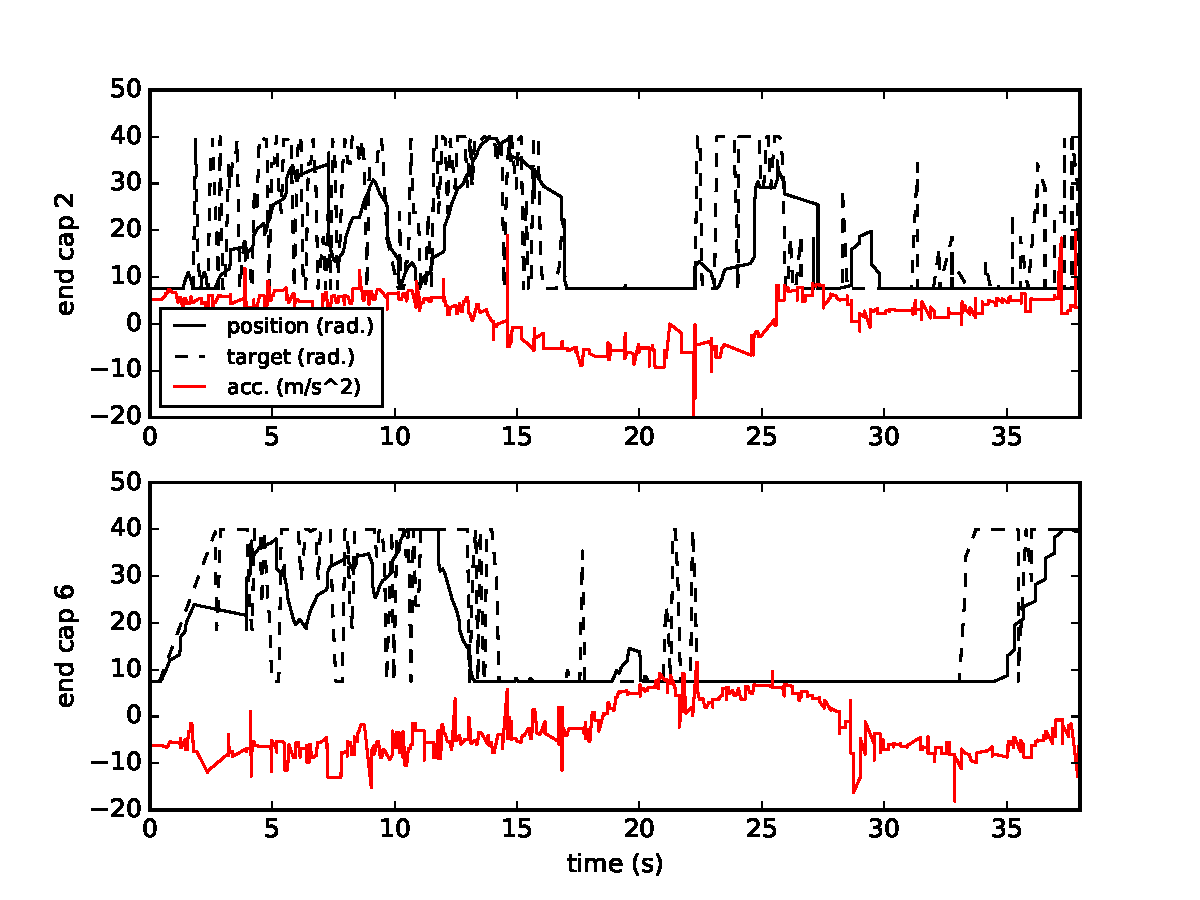
\includegraphics[width=\linewidth]{tex/img/plot_motor}
    \caption{
        \label{fig:commands}
        This plot shows actual motor positions, target motor positions, and 
        single axis accelerometer data over the first 40 seconds of a trial
        for two rod ends which are not connected via cables and not attached
        to the same rod. The commanded positions change based on
        the accelerometer feedback, showing the controller working as the robot
        changes orientation by rolling. The actual motor position  
        lags behind the target motor position due to motor dynamics and network UDP packet loss.
    }
\end{figure}

The open-loop policy was not able to produce any reasonable behavior on the real
robot, and we ran it only once due to concerns about hardware safety. 
%The lack
%of performance and safety exhibited by this policy can be explained by viewing
%the difference in motor commands sent by the learned policy in simulation and on
%the real robot, shown in Figure~\ref{fig:commands}. 
Due to various modeling
imprecisions, the simulated \SB{} has a greater maximum motor velocity, and the
policy uses this discrepancy to achieve faster locomotion. The open-loop policy
attempts to mimic this on the real robot, which does not work because the robot
cannot reach the same motor positions over a fixed number of time steps as in
simulation. 
%In addition, despite following all of the action constraints, the
%open-loop policy is dangerous for the cables because they are frayed by the
%constant expansion and contraction. 
%and we can see that it
%adopts a strategy that applies motor commands for a longer period of time in
%order to move the robot into the desired configuration and produce a successful
%locomotion gait.


% \section{CPG or Other Controller}
% \label{cpg_controller}

% \section{Dynamic Rolling}
% \label{dyncamic_rolling}